\documentclass[a4paper,12pt]{article}

\usepackage[utf8]{inputenc}
\usepackage{geometry}
\usepackage{graphicx}
\usepackage{amsmath}
\usepackage{hyperref}

\geometry{margin=1in}

\title{Electronics Experiment Report: Diode Characteristics}
\author{B13901165張勝勛, B13901087洪秉軒}
\date{\today}

% Language and font packages
\usepackage{ctex} % Chinese support

% Pseudocode and algorithm packages
% \usepackage{algorithm2e} % Advanced algorithm writing
% \usepackage{algpseudocode} % Pseudocode environment for algorithms

% Fancy style packages
\usepackage{fancyhdr} % Custom headers/footers
\usepackage{color} % Color support
\usepackage{xcolor} % Extended color support
\usepackage{tcolorbox} % Colored boxes
\usepackage{framed} % Framed environments

% Math and symbol packages
\usepackage{amsfonts}
\usepackage{amssymb}
\usepackage{mathtools}

% Table and figure packages
% \usepackage{booktabs} % Professional tables
% \usepackage{multirow} % Multi-row tables
% \usepackage{caption} % Custom captions
\usepackage{subcaption} % Subfigures

% Miscellaneous
\usepackage{enumitem} % Custom lists
\usepackage{listings} % Code listings
\usepackage{tikz} % Drawing diagrams
\usepackage{pgfplots} % For plotting graphs
\usepackage{float}

\begin{document}

\maketitle

\section{Experiment setup}
\begin{figure}[H]
    \centering
    
\includegraphics[width=0.8\textwidth]{exp_setup.png}
    \caption{Experiment setup}
    \label{fig:example}
\end{figure}
In this experiment, we set up a Common Source Amplifier circuit using an N-channel MOSFET.
Our goal is to analyze the DC and AC characteristics of the amplifier, including voltage, current and gain.\\
The parameters used in the experiment are as follows:
\begin{table}[H]
    \centering
    \begin{tabular}{|c|c|}
        \hline
        Parameter & Value \\
        \hline
        $V_{DD}$ & 15V \\
        $R_{G1}$, $R_{G2}$ & 1M$\Omega$ \\
        $R_D$, $R_S$, $R_L$ & 10k$\Omega$ \\
        $R_{sig}$ & 10k$\Omega$ \\
        $C_{C2}$, $C_S$ & 0.1$\mu$F(104) \\
        $C_{C1}$ & 0.01$\mu$F(103) \\
        $V_{sig}$ & 200mV (AC) \\
        Frequency & 200Hz to 500kHz \\
        \hline
    \end{tabular}
    \caption{Experiment Parameters}
    \label{tab:parameters}
\end{table}
\section{DC result}
\subsection{Measured Values}
\begin{table}[H]
    \centering
    \begin{tabular}{|c|c|c|}
        \hline
        Parameter & Measured Value & Description \\
        \hline
        $V_G$ & 7.188V & about half of $V_{DD}$  = 15V/2 = 7.5V\\
        $V_D$ & 9.59V & higher than $V_G$, working at saturation region\\
        $V_S$ & 5.408V & \\
        $I_G$ & 0.002mA & about 0 since no current at gate\\
        $I_D$ & 0.544mA & same as $I_S$ \\
        $I_S$ & 0.544mA & same as $I_D$ \\
        \hline
    \end{tabular}
    \caption{DC Measurement Results}
    \label{tab:dc_results}
\end{table}
\section{AC result}
In this section, we present the voltage gain results of the amp at $f = 1kHz$.
\begin{table}[H]
    \centering
    \begin{tabular}{|c|c|}
        \hline
        Condition & Measured Gain \\
        \hline
        With $C_S$, $v_o$ vs $v_{sig}$ & 2.03 \\
        With $C_S$, $v_o$ vs $v_i$ & 2.21 \\
        Without $C_S$, $v_o$ vs $v_{sig}$& 0.43 \\
        \hline
    \end{tabular}
    \caption{AC Measurement Results at $f = 1kHz$}
    \label{tab:ac_results}
\end{table}
\section{Pictures}
\begin{figure}[H]
    \centering
    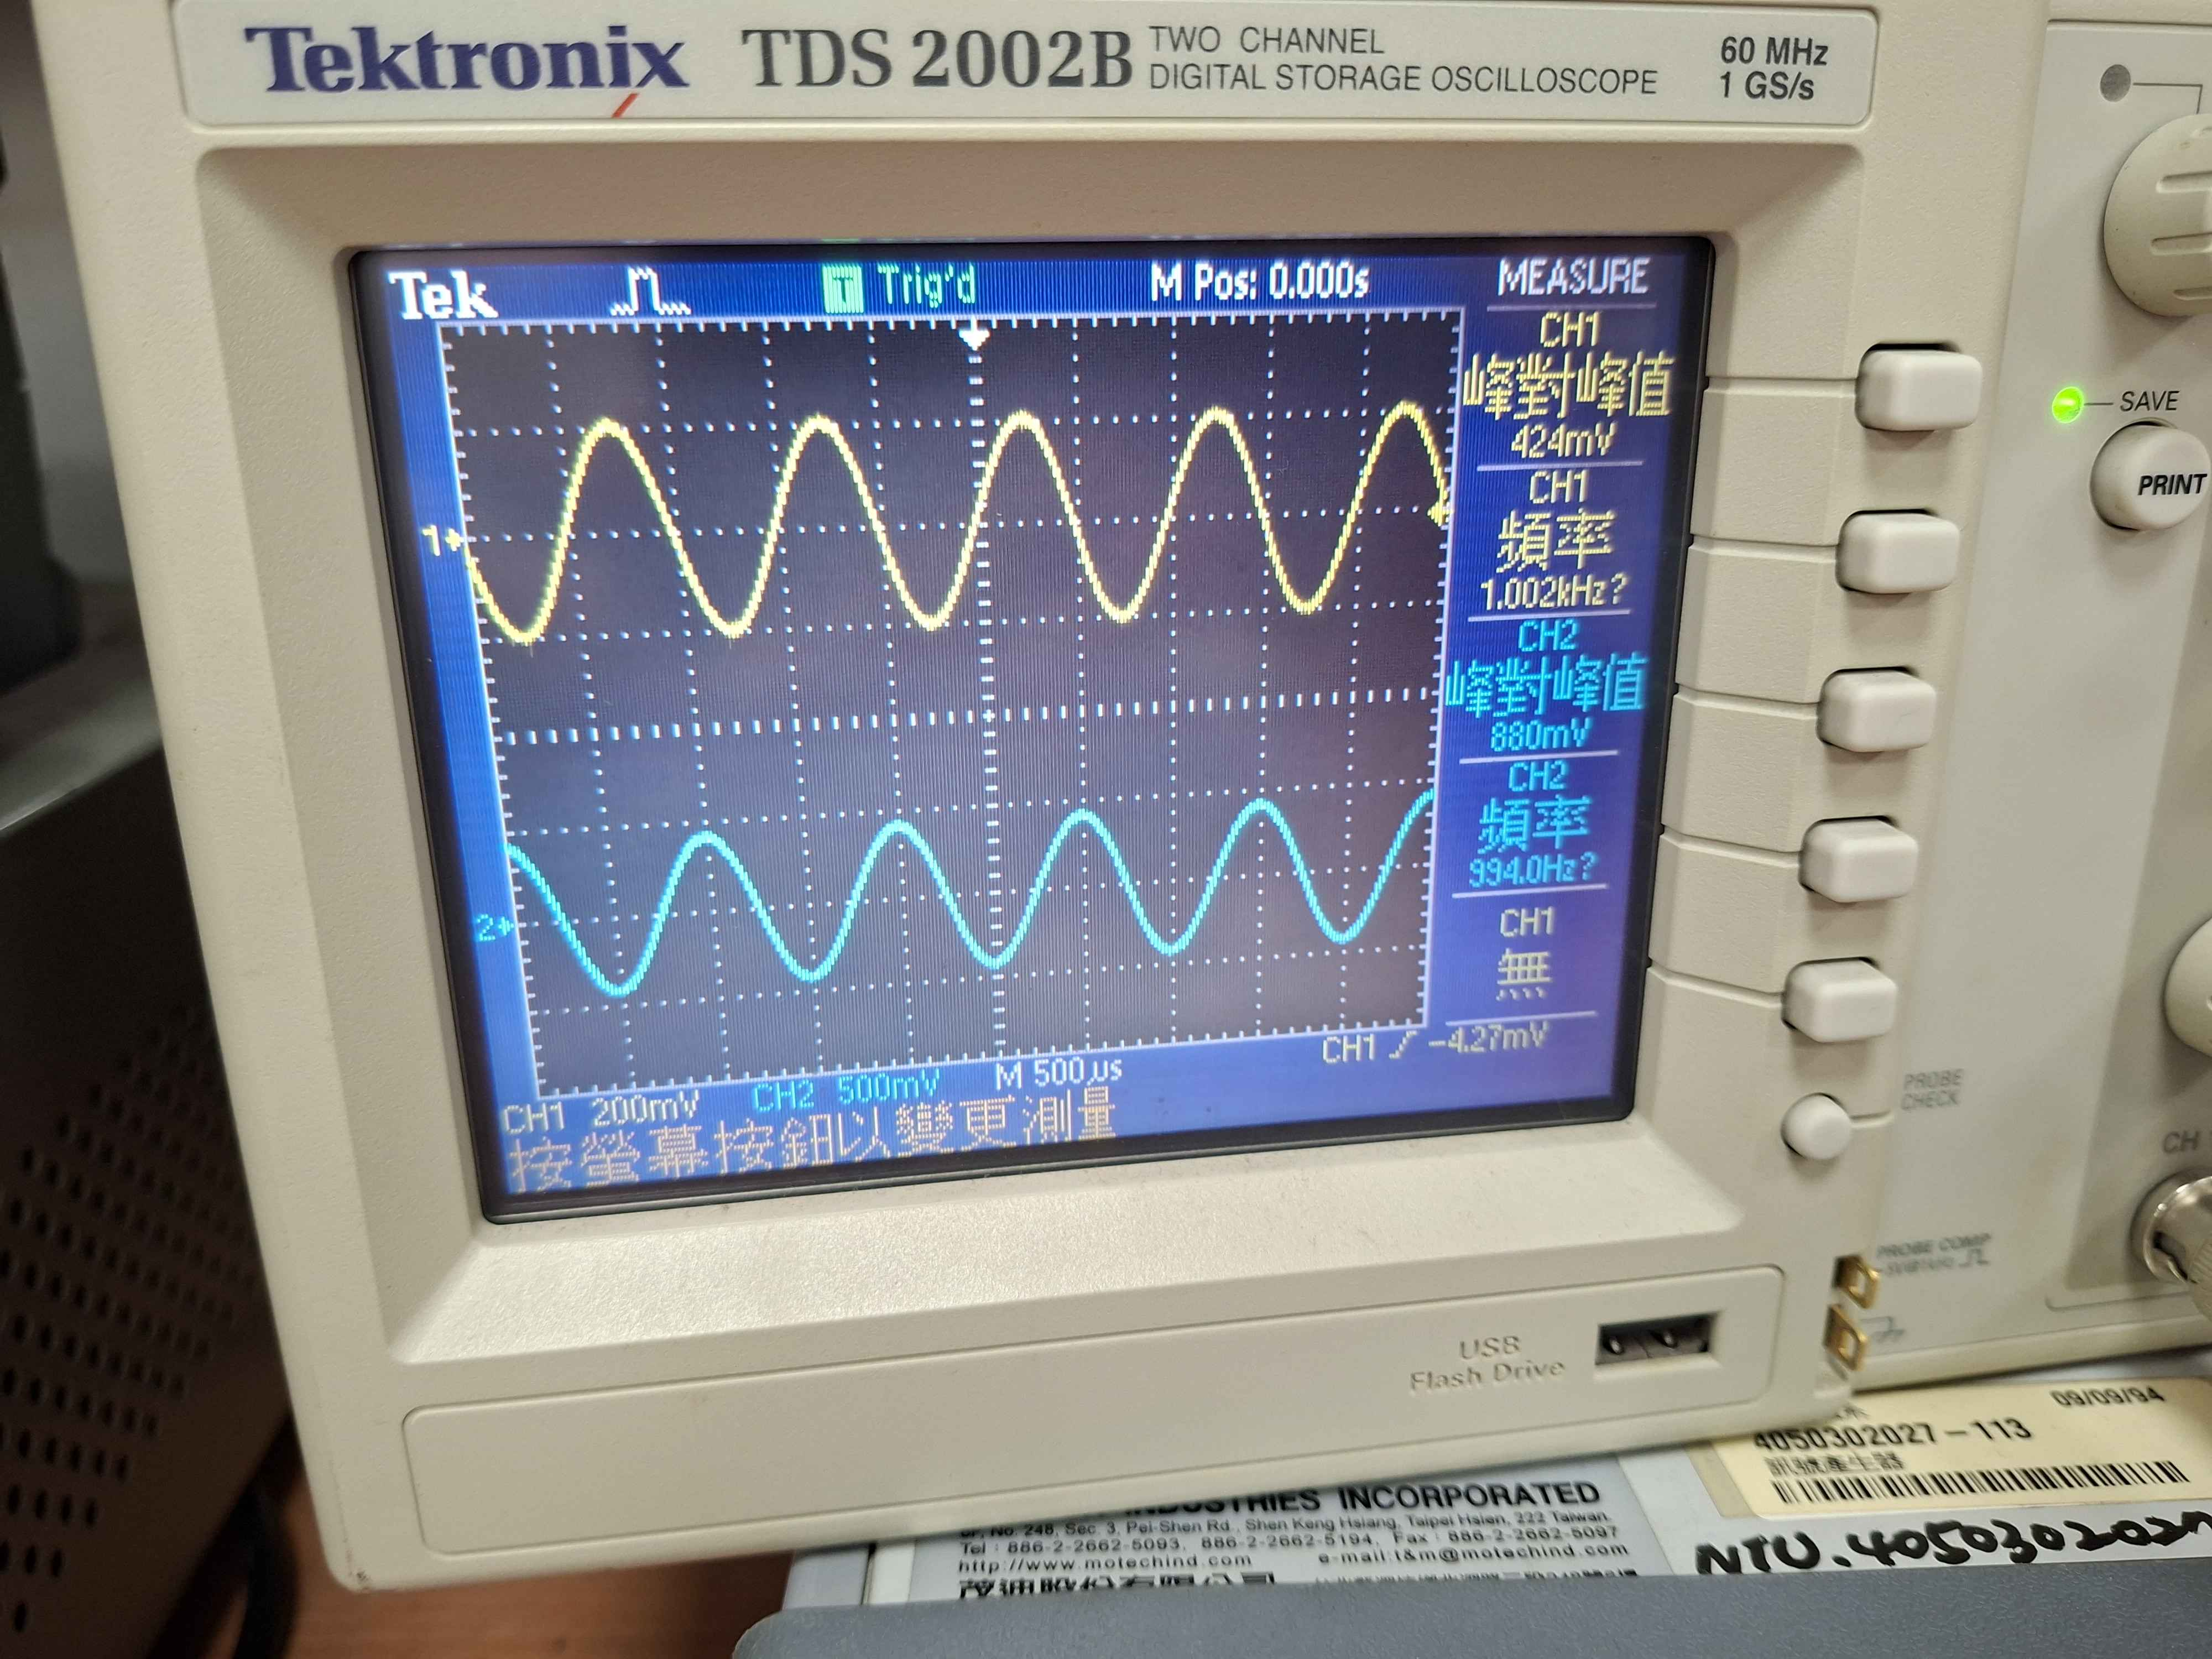
\includegraphics[width=0.8\textwidth]{exp_1.jpg}
    \caption{$v_o / v_{sig}$ with $C_s$}
    \label{fig:example}
\end{figure}

\begin{figure}[H]
    \centering
    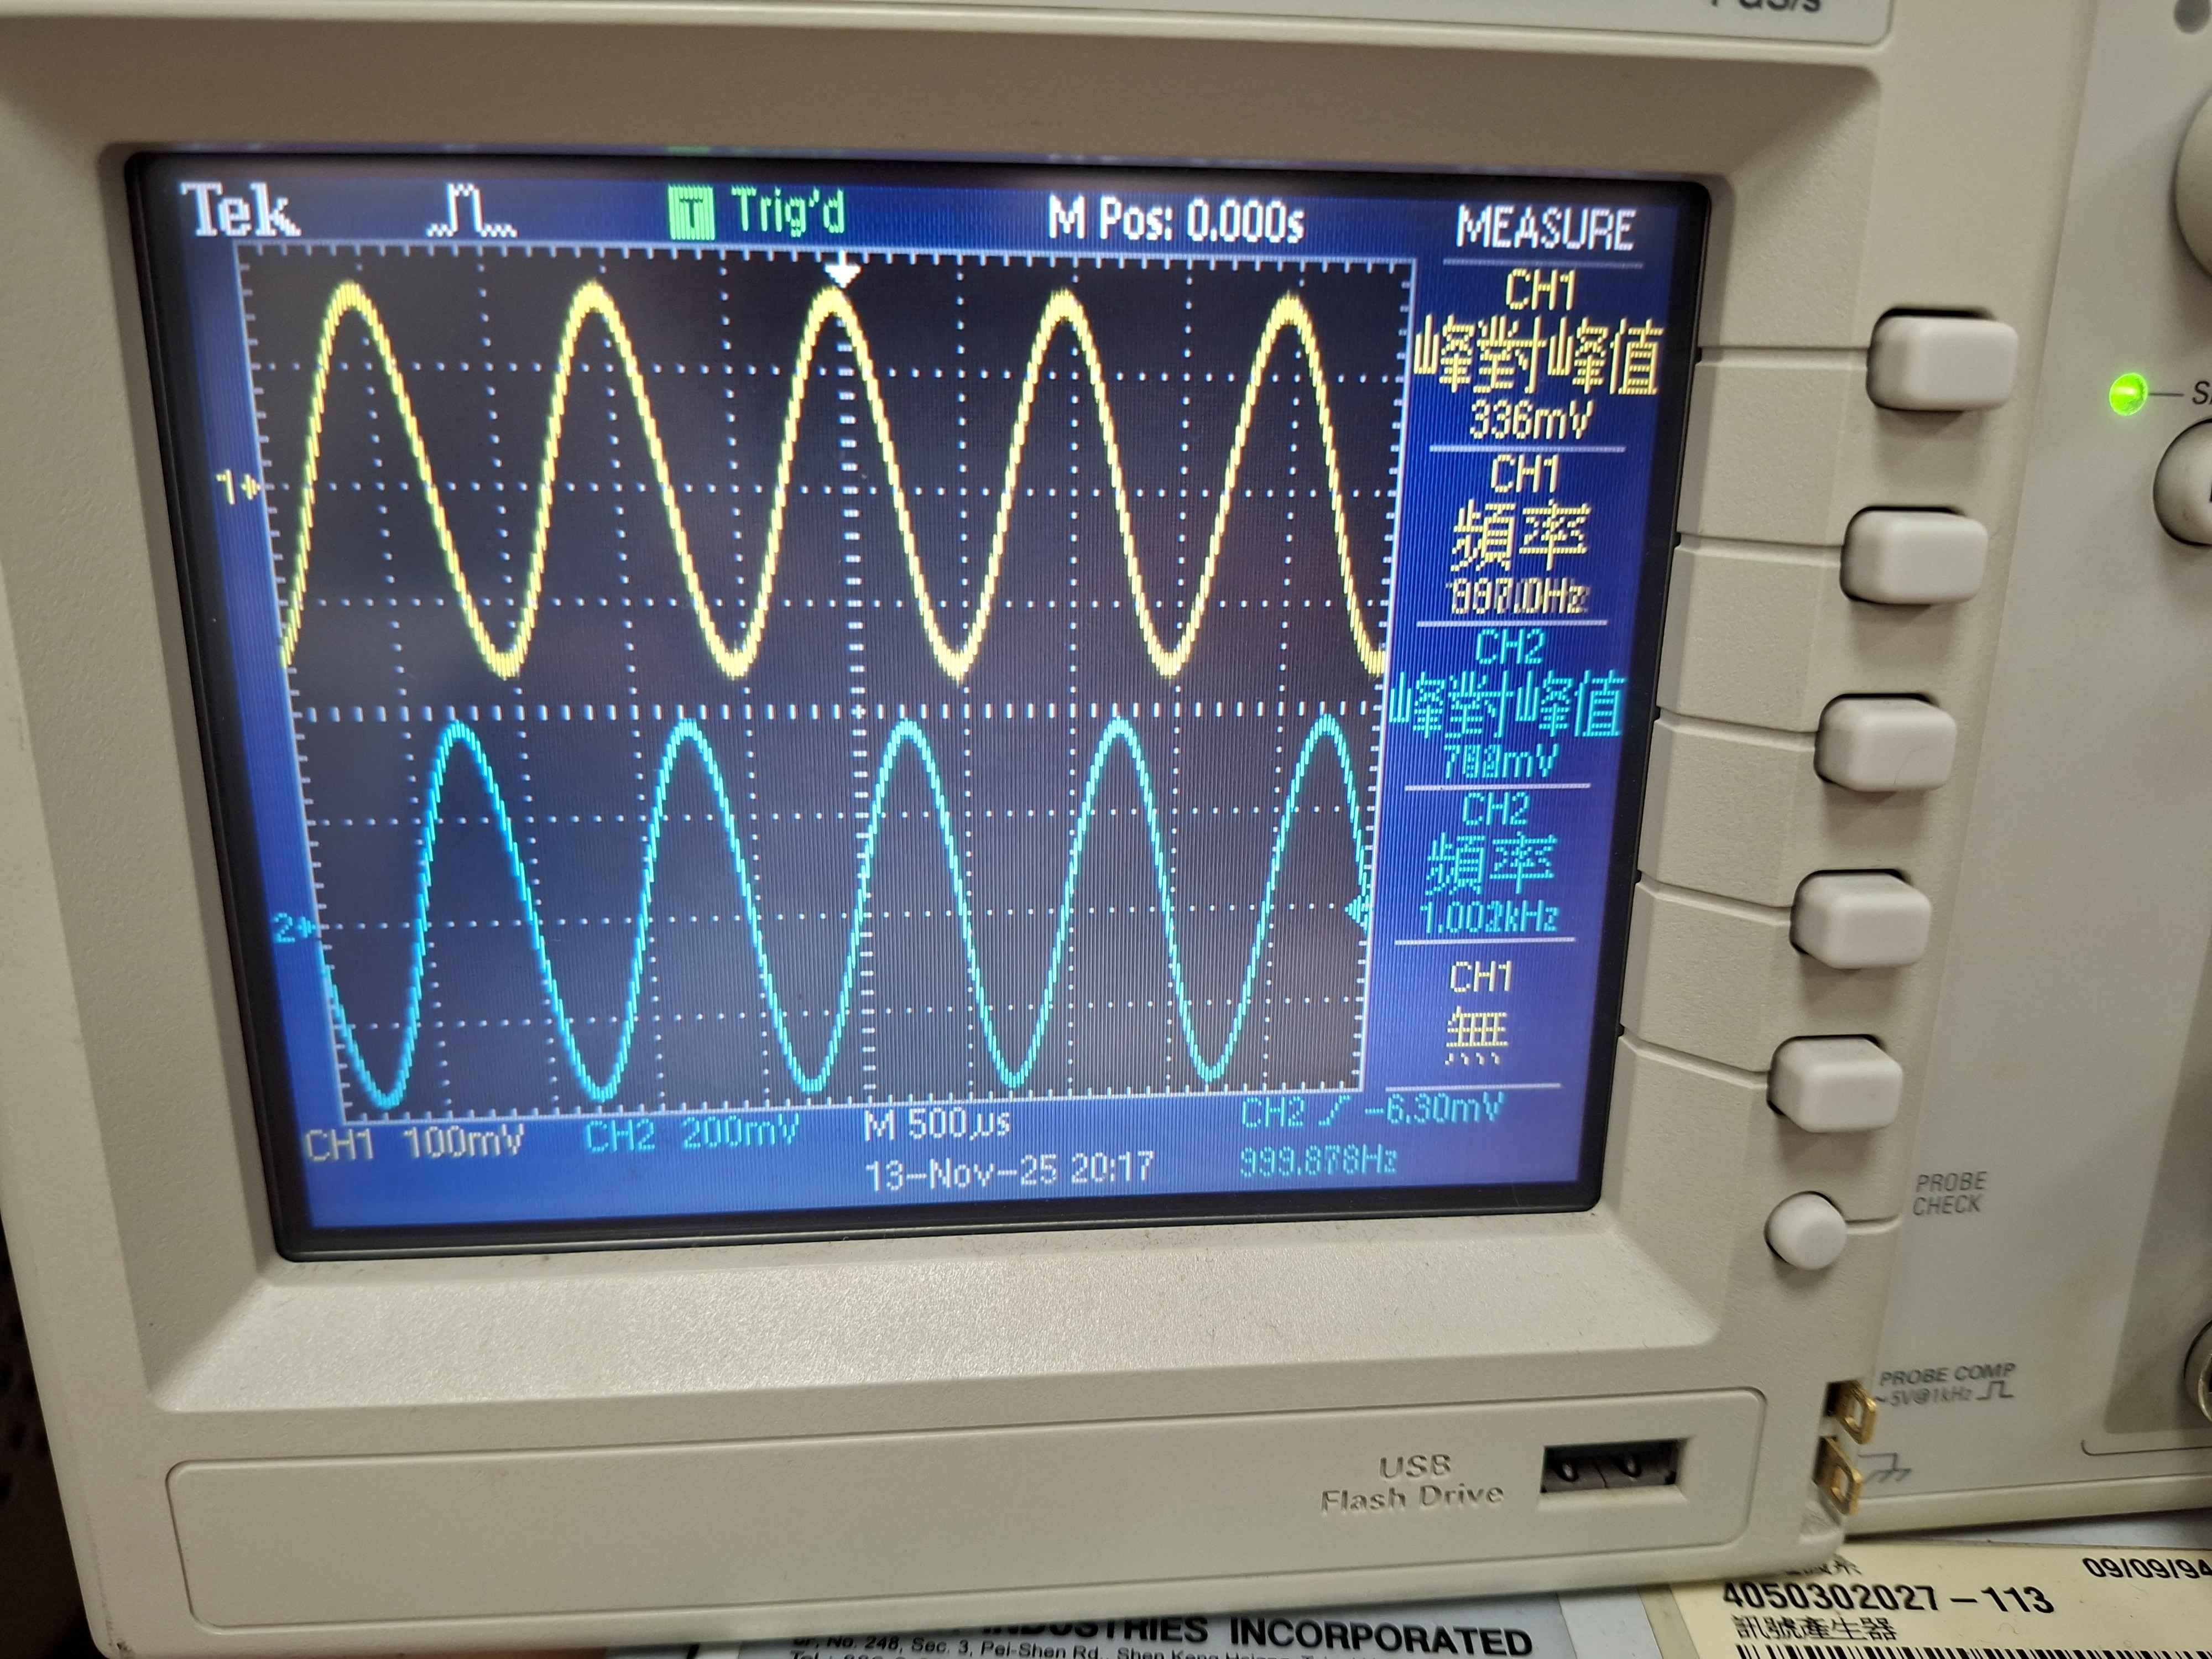
\includegraphics[width=0.8\textwidth]{exp_2.jpg}
    \caption{$v_o / v_i$ with $C_s$}
    \label{fig:example}
\end{figure}

\begin{figure}[H]
    \centering
    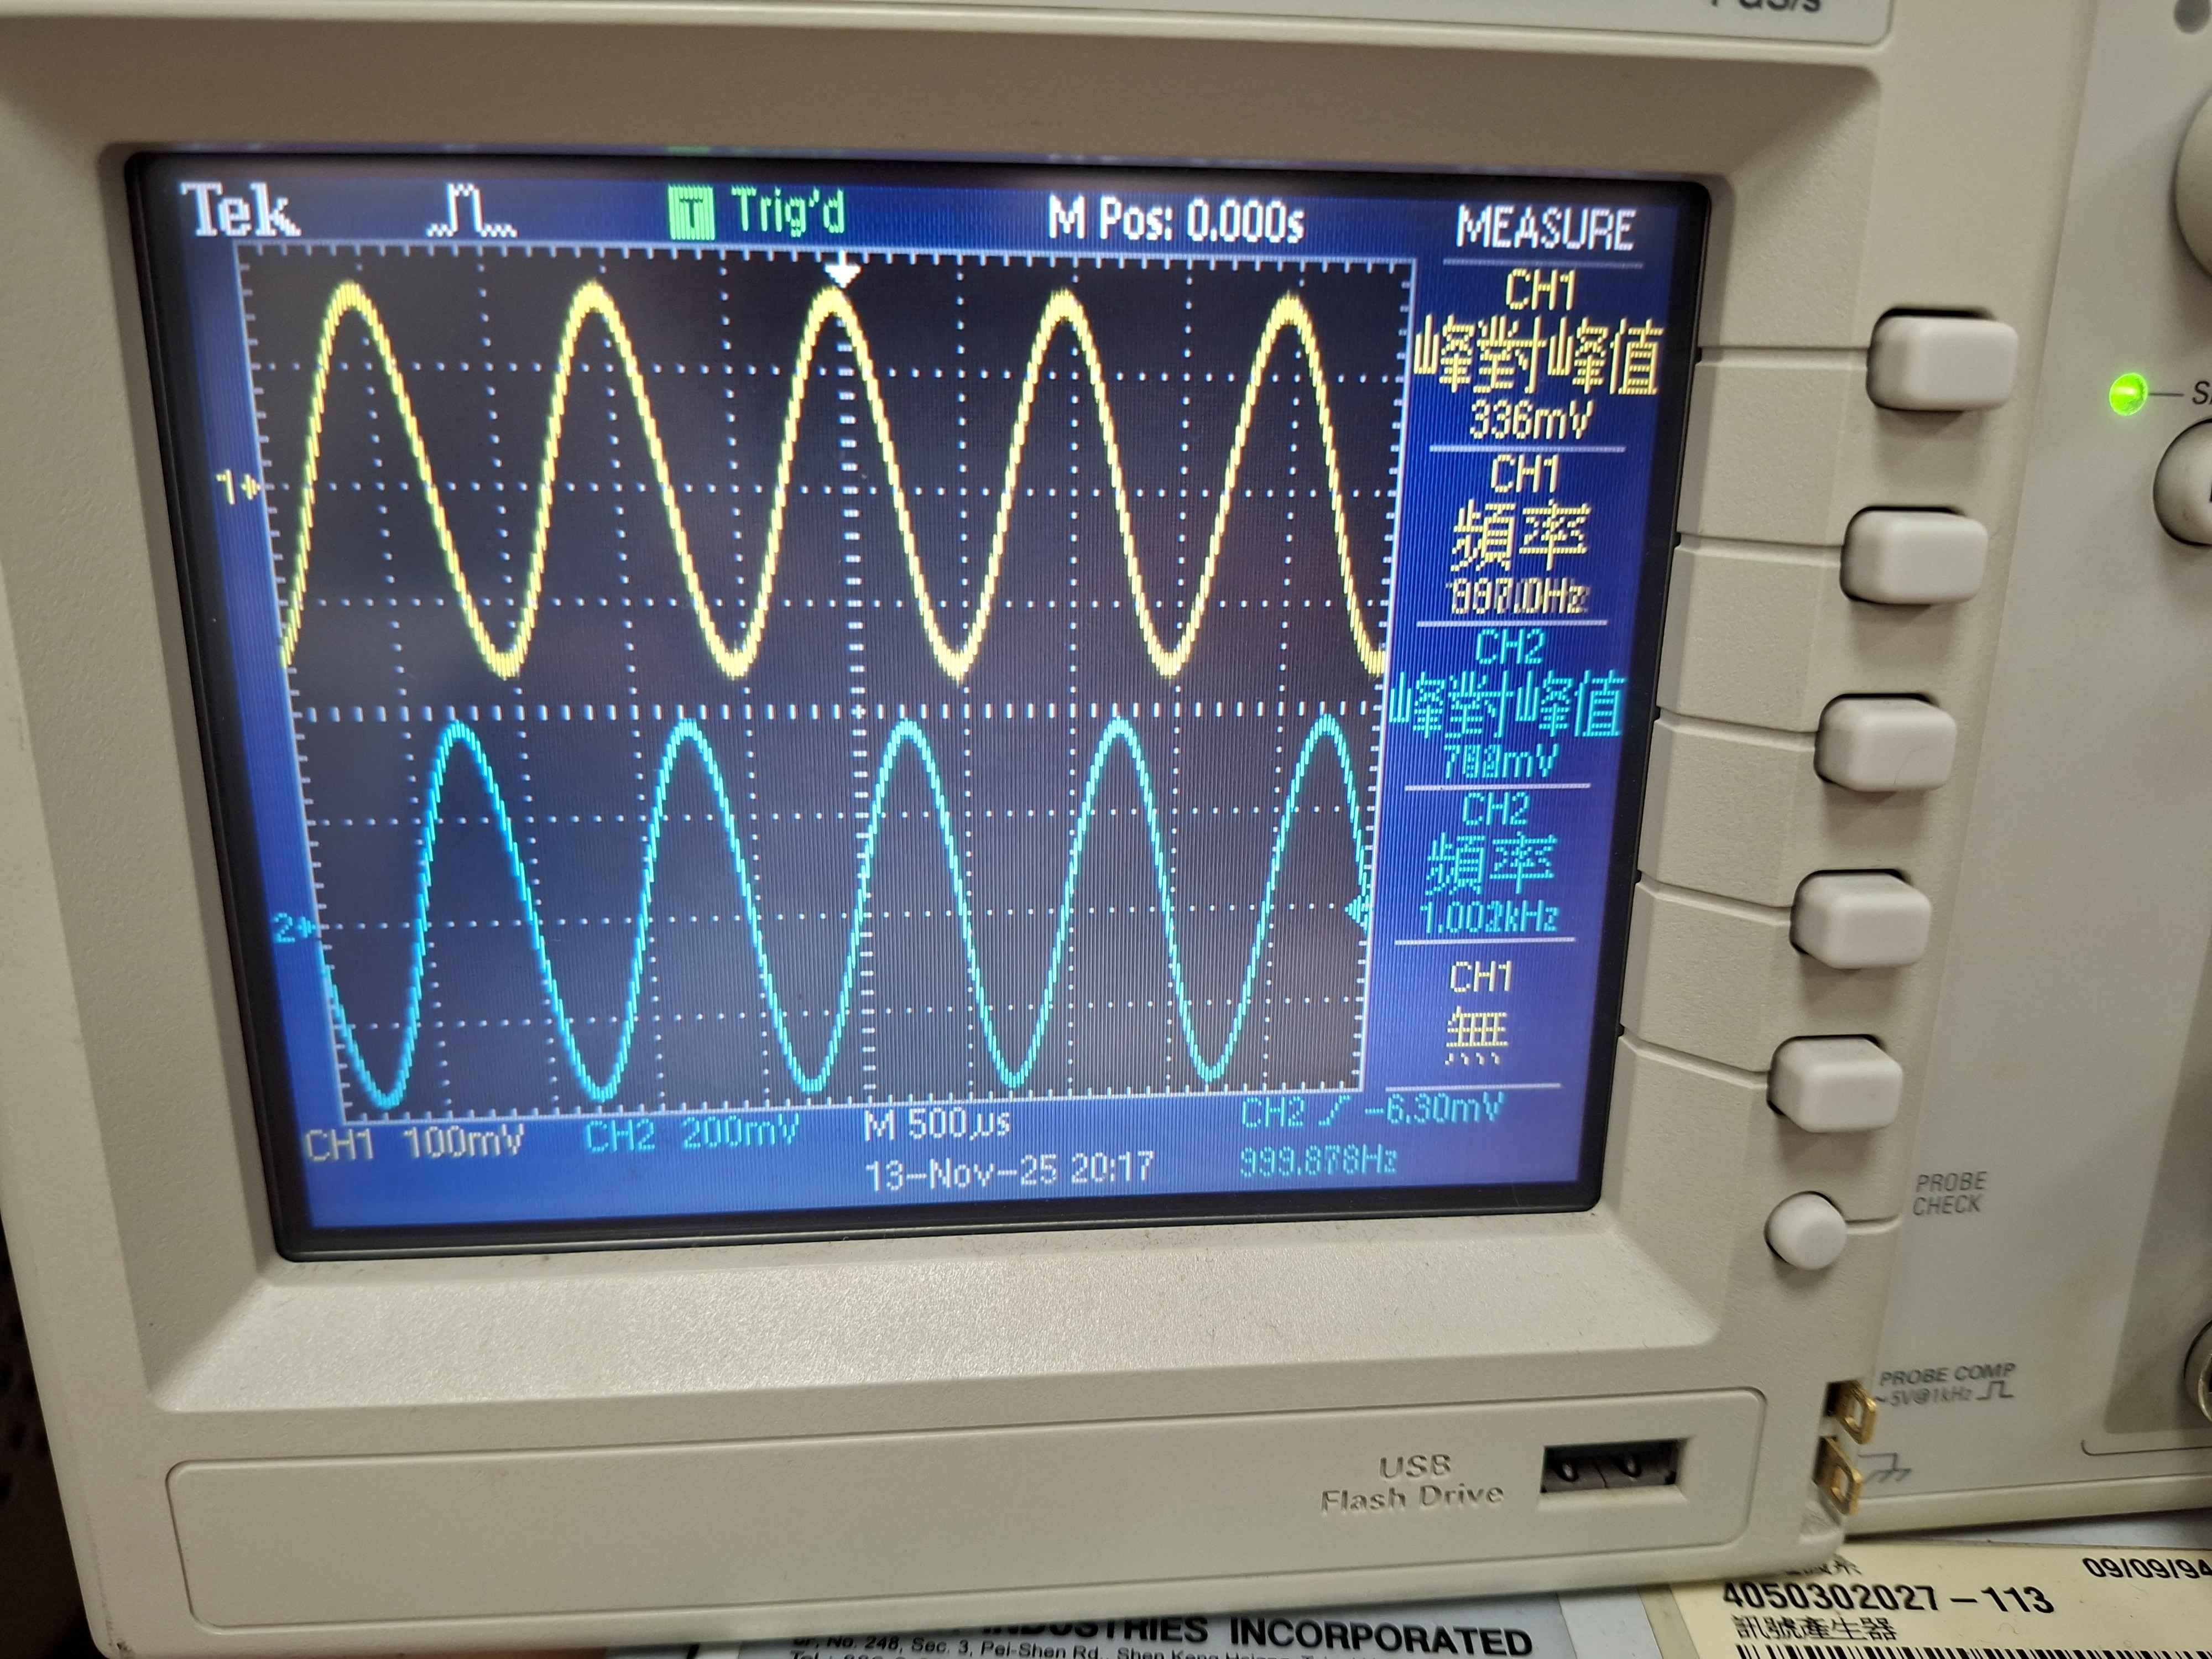
\includegraphics[width=0.8\textwidth]{exp_2.jpg}
    \caption{$v_o / v_{wig}$ w/o $C_s$}
    \label{fig:example}
\end{figure}

\end{document}